\beginsong{Zeit zum Handeln}[
    wuw={Kilian Hähn, Jonas Höchst, Matthias \emph{Atze} Müller, Ann-Kathrin Pullmann}, 
    lager={VCP Hessen Landeslager 2016 \emph{''H{\ae}sseh\=aven''}}, 
    index={Wir standen allein in der weiten Welt}, 
    jahr={2016},
    ]

\beginverse
\endverse
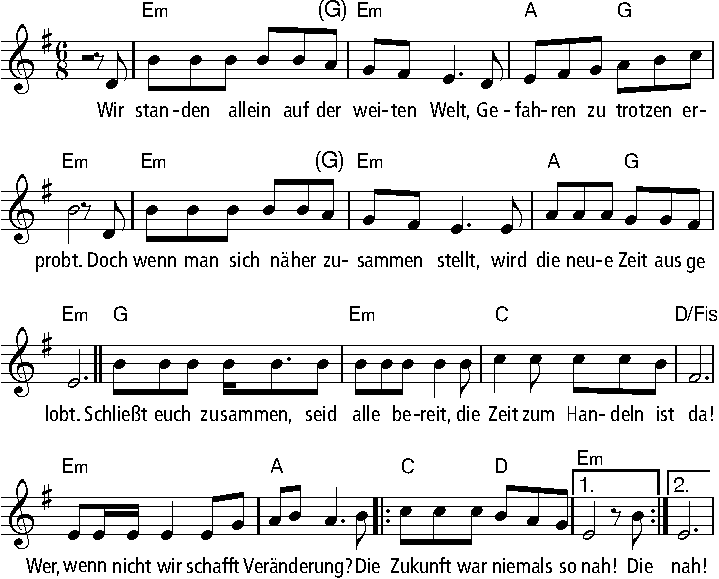
\includegraphics[page=1]{Noten/Zeit-zum-Handeln-crop.pdf}

\renewcommand{\everychorus}{\textnote{}}
\beginchorus
\nolyrics{\[Zwischenspiel:] \[Em] \[A] \[G] \[Em]}
\endchorus

\beginverse
\[Em]Mitbringen wir dann \[(G)]so \[Em]manchen Tand; und \[A]Tücher und \[G]Pfeffer und \[Em]Tee,
haben \[Em]manche zum ersten \[(G)]Mal \[Em]{in der} Hand: Be\[A]zahlt - Segel \[G]setzen - Ad\[Em]e! \[D]
\endverse

\renewcommand{\everychorus}{\textnote{\bf Refrain}}
\beginchorus 
\[G]Schließt euch zusammen, seid \[Em]alle bereit, die \[C]Zeit zum Handeln ist \[D/F#]da!
\[Em]Wer, wenn nicht wir schafft Ver\[A]änderung? \lrep Die \[C]Zukunft war \[D]niemals so \[Em]nah! \rrep
% \nolyrics{\[Zwischenspiel:] \[Em] \[A] \[G] \[Em]}
\endchorus

\renewcommand{\everychorus}{\textnote{}}
\beginchorus
\nolyrics{\[Zwischenspiel:] \[Em] \[A] \[G] \[Em]}
\endchorus

\beginverse
Von ^Gödecke Michels ^be^raten, ver^folgt man uns ^über das ^Meer.
Doch ^wir, wir riechen ^den ^Braten und ^machen's den ^Freibeutern ^schwer! ^
\endverse

\renewcommand{\everychorus}{\textnote{\bf Refrain (wdh.)}}
\beginchorus
% \nolyrics{\[Zwischenspiel:] \[Em] \[A] \[G] \[Em]}
\endchorus

\renewcommand{\everychorus}{\textnote{\bf Übergang}}
\beginchorus
\endchorus

\centering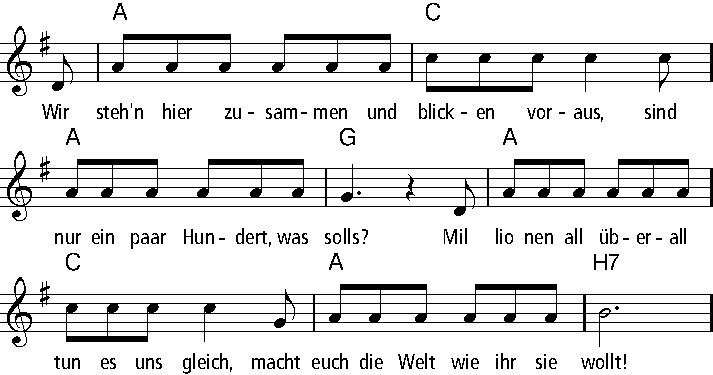
\includegraphics[width=1\textwidth]{Noten/Zeit-zum-Handeln-C-crop.pdf}	

\renewcommand{\everychorus}{\textnote{\bf Refrain}}
\beginchorus 
\lrep \[G]Schließt euch zusammen, seid \[Em]allzeit bereit, die \[C]Zeit zum Handeln ist \[D/F#]da!
\[Em]Unsere Welt, sie ist \[A]uns geweiht, die \[C]Zukunft war \[D]niemals so \[Em]nah! \rrep
Nein, die \[C]Zukunft war \[D]niemals so \[Em]nah!
\endchorus


\endsong

\beginscripture{}
Das Lied wurde auf einem V-Team in abendlicher Runde geschrieben und auf der LV 2016 zum Lagerlied des hessischen Landeslagers 2016 ''H{\ae}sseh\=aven'' gewählt.
\endscripture